\documentclass[handout]{beamer}

\usepackage{Haust2017glærur}

\title{Tölvunarfræði 1a}
\subtitle{Vika 7, seinni fyrirlestur}

\begin{document}

\begin{frame}
\titlepage
\end{frame}

\section{Inngangur}

\begin{frame}{Í síðasta þætti\ldots}
\begin{itemize}
 \item Strengir
\end{itemize}
Kafli: 7 
\end{frame}

\section{Eval og tölvuhögun}

\begin{frame}[fragile]{Eval}
Fallið \texttt{eval} framkvæmir streng sem Matlab-skipun.

\begin{minted}[frame=lines]{matlab}
>> eval('a = 1:4')
a =
   1   2   3   4
>> eval('x = 1:5; s = sum(x)') % Röð skipana
s =  15
\end{minted}

Hægt er að keyra heilu forritin á þennan hátt.
\end{frame}

\begin{frame}[fragile]{Notkunardæmi á \texttt{eval}}
Getum látið notanda slá inn fall til að teikna:
\begin{minted}[frame=lines]{matlab}
f = input('Sláið inn fall (af x): ','s');
x = 0:0.1:10;
plot(x, eval(f))
\end{minted}
\end{frame}

\begin{frame}{Hvenær skal ekki nota eval}
\begin{itemize}
 \item Oftast er slæm hugmynd að nota \texttt{eval}!
 \begin{itemize}
  \item Reyna aðra möguleika fyrst
  \item Getur engu að síður verið einfaldara en aðrir möguleikar
 \end{itemize}
 \item \texttt{eval} er ekki hraðvirkt
 \item Sé notanda leyft að skrifa og keyra kóða er það öryggisgalli
 \begin{itemize}
  \item Gæti skipt máli í Matlab sé kóði keyrður á vél með marga notendur
  \item Sískemmtilegt gúgl: ``Arbitrary code execution'' 
 \end{itemize}
\end{itemize}
\end{frame}

\subsection{Forrit sem gögn}

\begin{frame}{Forrit sem gögn}
\begin{itemize}
 \item Þetta vekur athygli á mikilvægu atriði
 \begin{itemize}
  \item Þó að \emph{forrit} og \emph{gögn} séu aðskilin hugtök, þá meðhöndlar tölvan þau á sama hátt
  \begin{itemize}
   \item Forrit hafa stýriskipanir sem geta breytt hegðun forritsins
   \item En forrit geta líka breytt forritum
  \end{itemize}
  \item Afleiðingar:
  \begin{itemize}
   \item Tölvur ráða við mjög margvísleg verkefni
   \item Auðvelt er að breyta hegðun tölva
  \end{itemize}
 \end{itemize}
\end{itemize}
\end{frame}

\begin{frame}{ENIAC}
\begin{center}
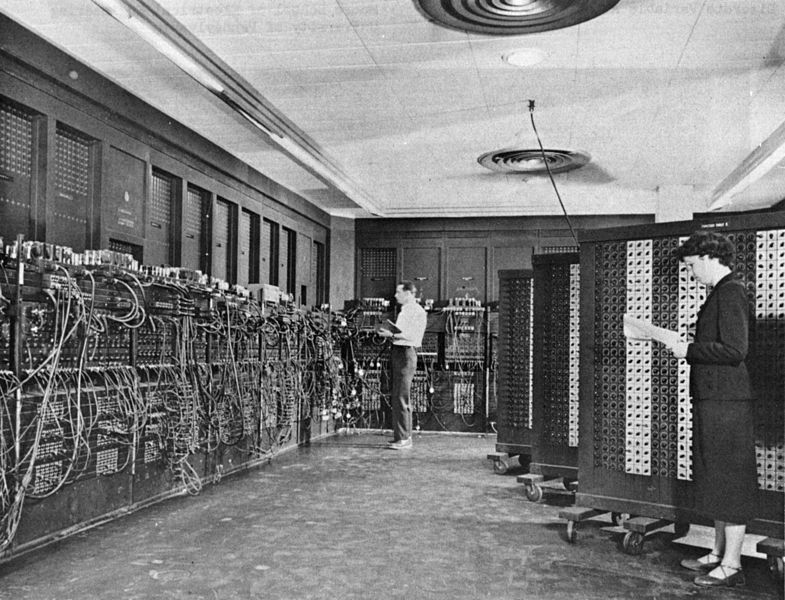
\includegraphics[width=0.8\textwidth]{Pics/eniac}
\end{center}
\end{frame}

\begin{frame}{John von Neumann}
\begin{columns}
\column{0.7\textwidth}
\begin{itemize}
 \item Von Neumann var gríðarlega afkastamikill vísindamaður
 \begin{itemize}
  \item 150 útgefnar greinar, flestar í stærðfræði
  \item \href{https://en.wikipedia.org/wiki/List\_of\_things\_named\_after\_John\_von\_Neumann}{List of things named after John von Neumann}
 \end{itemize}
 \item Setti fram hugmyndina um að geyma forrit í minni tölvunnar eins og hver önnur gögn
 \begin{itemize}
  \item Þetta er hluti af \emph{von Neumann högun} tölva
  \item Nær allar tölvur síðan hafa haft þetta skipulag
 \end{itemize}
\end{itemize}
\column{0.3\textwidth}
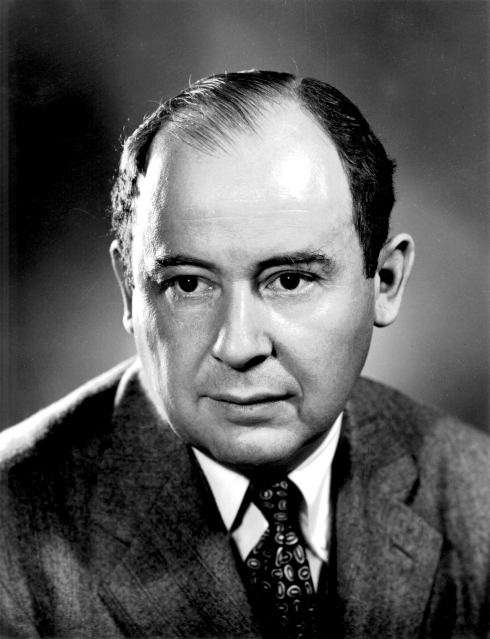
\includegraphics[width=\linewidth]{Pics/john-von-neumann}

John von Neumann (1903-1957)
\end{columns}
\end{frame}

\section{Meira um strengi}

\begin{frame}[fragile]{\texttt{isstrprop} fallið}
\vspace{1.5\baselineskip}
Getum notað fallið \texttt{istrpprop} til að athuga hvort að stafir strengs séu af ákveðinni gerð\footnote{Fleiri möguleikar eru til. Sjá \texttt{help isstrprop}.}.
\begin{minted}[frame=lines]{matlab}
>> isstrprop('Jón', 'lower')
ans =
   0   1   1
>> isstrprop('Ha!?','punct')
ans =
   0   0   1   1
>> isstrprop('a b ','wspace') % Whitespace, biltákn
ans =
   0   1   0   1
\end{minted}
\end{frame}

\begin{frame}[fragile]{Fallið \texttt{mat2str}}
Fallið \texttt{mat2str} getur breytt fylki í streng sem skilgreinir fylkið.
\begin{minted}[frame=lines]{matlab}
>> a = randi(10, 2, 2)
a =
   5   6
   4   3
>> mat2str(a)
ans = [5 6;4 3]
\end{minted}
\end{frame}

\begin{frame}[fragile]{Meira um \texttt{sprintf}}
\begin{itemize}
 \item Við getum notað \texttt{sprintf} til að fá tölur á ákveðnu sniði
 \begin{itemize}
  \item \texttt{fprintf} dugar líka ef við viljum einungis \emph{sýna} töluna, en ekki geyma hana
 \end{itemize}
\end{itemize}
\begin{minted}[frame=lines]{matlab}
>> sprintf('%6.4f',48.2)
ans =
48.2000
\end{minted}
\end{frame}

\begin{frame}[fragile]{\texttt{sprintf} í lykkju}
Dæmi: Notkun \texttt{sprintf} til að búa til strengjafylki

\begin{minted}[frame=lines]{matlab}
usernames = [];
for i = 9:11
  usernames = [usernames; sprintf('jon%-2d',i)];
end
disp(usernames)
\end{minted}
Útkoman:\pause $3\times 5$ strengjafylki.
\end{frame}

\begin{frame}[fragile]{Oft gagnlegt: Að skipta upp streng}
\begin{itemize}
  \item \texttt{strtok} skiptir streng upp í tvo búta, ``haus'' og ``hala''
  \begin{itemize}
   \item Leitar að ``skiptitákni'' - allt sem er fyrir framan táknið er hausinn, afgangur strengsins er halinn
   \begin{itemize}
       \item Undantekning: Skiptitákn fremst í strengnum eru hunsuð
   \end{itemize}
   \item Sjálfgefið skiptitákn er bilstafur
  \end{itemize}
\end{itemize}
\begin{minted}[frame=lines]{matlab}
>> [haus, hali] = strtok('Fyrsta annað þriðja')
haus =
Fyrsta
hali =
 annað þriðja
\end{minted}

\end{frame}


\begin{frame}{Fyrirlestraræfing}
    \begin{enumerate}
        \item Hvað gerir eftirfarandi skipun?\\
        \texttt{eval('eval(''b = 4'')')}
        \item Notið vigurkóðun og \texttt{isstrprop} fallið til að hreinsa allt nema tölur úr strengnum \texttt{s}.
        \item Notið \texttt{strtok} fallið til að skipta strengnum \texttt{'Fyrsta annað þriðja'} niður í þrjár aðskildar breytur.
    \end{enumerate}
\end{frame}

\section{Miðmisserispróf}

\begin{frame}{Námsefni til miðmisserisprófs}
\begin{itemize}
 \item Glærur
 \item Verkefni (sérstaklega skilaverkefni)
 \item Kaflar 1-7 í kennslubókinni (fjórðu útgáfu), með undantekningum:
 \begin{itemize}
  \item Kafli 3.8 (föll sem skipanir)
  \item \texttt{menu}-fallið (bls.133)
  \item Kafli 6.3 (\texttt{menu} + einingaforritun)
  \item Kafli 6.4.1 (\texttt{persistent} breytur)
  \item Kafli 6.5 (aflúsun - fórum yfir, en er ekki til prófs)
 \end{itemize}
\end{itemize}
\end{frame}

\begin{frame}{Grófur efnislisti}
\begin{columns}
\column{0.5\textwidth}
\begin{itemize}
 \item Matlab segðir og breytur
 \item Vigrar og fylki
 \item Föll og skipanaskrár
 \item \texttt{if}, \texttt{elseif} og \texttt{else}
 \item Lykkjur (\texttt{for} og \texttt{while})
 \item Vigurkóðun
 \item Inntak og úttak
 \item Gagnagerðir
 \begin{itemize}
  \item Heiltölur, fleytitölur, rökbreytur og stafir
 \end{itemize}
\end{itemize}
\column{0.5\textwidth}
\begin{itemize}
 \item Tvíundarkerfið
 \item Línurit
 \item Skráarvinnsla: \texttt{save} og \texttt{load}
 \item Gildissvið breyta
 \item \texttt{switch}
 \item Þýðing/túlkun og fleira undir húddinu
 \item Skipulag forrita
 \item Ýmis sérhæfð föll
\end{itemize}
\end{columns}
\end{frame}


\end{document}
